% This is file NWSguide.tex
% release v1.00, 12th June 2012
%   (based on JFPguide.tex v1.11 for LaTeX 2.09)
% Copyright (C) 2012 Cambridge University Press

\NeedsTeXFormat{LaTeX2e}

\documentclass{nws}

%%% Macros for the guide only %%%
\providecommand\AMSLaTeX{AMS\,\LaTeX}
\newcommand\eg{\emph{e.g.}\ }
\newcommand\etc{\emph{etc.}}
\newcommand\bcmdtab{\noindent\bgroup\tabcolsep=0pt%
  \begin{tabular}{@{}p{10pc}@{}p{20pc}@{}}}
\newcommand\ecmdtab{\end{tabular}\egroup}
\newcommand\rch[1]{$\longrightarrow\rlap{$#1$}$\hspace{1em}}
\newcommand\lra{\ensuremath{\quad\longrightarrow\quad}}

\title[Bridging or Bonding? Measures of Topic Centrality for Online Political Engagement]
      {Bridging or Bonding? Measures of Topic Centrality for Online Political Engagement}

 \author[C.J.K Raymond]
        {Cameron Raymond\\
        School of Computing, Queen's University, Kingston K7L 3N6, CA\\
         \email{c.raymond@queensu.ca}}

\jdate{May 2020}
\pubyear{2020}
\pagerange{\pageref{firstpage}--\pageref{lastpage}}
% \doi{S0956796801004857}

% \newtheorem{lemma}{Lemma}[section]

\begin{document}

\label{firstpage}

\maketitle

\begin{abstract}
  The advent of social media has enabled political parties to engage with the
  broader populous in new and unforeseen ways -- and the ability to bypass the
  traditional mediating forces of mass media allows for an unfiltered promotion
  of policy, ideology and party stances. Drawing on Twitter data leading up to
  the 2019 Canadian Federal Election, this paper develops two novel, graph-based methods that
  capture how different categories of messages drive different patterns of political
  engagement. Through the two proposed variations of topic centrality -- on which
  measures how central a topic was to the general discourse, and one which
  measures how central a topic was to a particular voting bloc -- statistically
  significant variations in topic centrality are then shown and discussed. %MORE_SPECIFIC
  \paragraph{Keywords:} \emph{centrality, political communication, social media, topic modeling}
\end{abstract}

\tableofcontents

\section{Introduction}

The way information is distributed and received has changed significantly over
the past decade. As Cogburn and Espinoza-Vasquez argue, Barrack Obama’s 2008
presidential campaign was a watershed moment in social media campaigning – and
in the subsequent decade, from Macron to Brexit to the Five Star Movement,
social media has played an increasing role in how politics is conducted
\cite{cogburn2011networked}.  The same holds true for Canada, between 2013 and
2018 the share of Canadian federal media expenditure spent on digital
advertising rose from 27\% to 65\%, a 140\% increase, making the study of new
media critical from a social science perspective
\cite{annualReportCanadaAdvertisingActivities_2018}. Over the past 12 years,
political elites have subverted traditional models of political communication by
using social media to directly promote various policies, topics and issues to
the electorate\footnote{The
terms policy, issue and topic will be used interchangeably to refer to
categories of messages.}\cite{mcnair2017introduction}.

Additionally, it is important to note that not all messages promoted by
political elites are likely to serve the same purpose. Some topics may be
logistical in nature, informing party affiliates of campaign events; other
topics may be promoted in an attempt to rally that party's core voting bloc;
others, finally, may be an attempt to attract
engagement from new, untapped demographics. The latter two categories are in
many ways analogous to Robert Putnam's conception of social capital
\cite{putnam2001social}. Here, Putnam draws the distinction between two forms
of social capital: bonding social capital, which occurs within a group -- and
bridging social capital, which unites different demographics
\cite{putnam2001social}. Therefore, the research question being proposed is:
are their data to support the notion that some political messages are bonding in
nature, rallying members within a group, while other political messages are
bridging in nature? This question will be answered within the context of the
2019 Canadian Federal Election with the Tweets of Canada’s five major, english
speaking party leaders: Andrew Scheer, Elizabeth May, Jagmeet Singh, Justin
Trudeau, and Maxime Bernier. 

In order to answer this question, a justification of Canadian politics and
social media data in this context will be given. Then an overview of the data
collected and a formal definition of the political engagement graph used will
allow for the exploration of two measures of topic centrality: total network
topic centrality, and party leader topic centrality. Finally, results from this
process and a discussion of their implications will highlight possibilities for
future research.  

\subsection{Social Media in the Canadian Context}

While it is clear that technology is changing how information is received, and
thus also changing how politics is conducted, it may not be clear the role of
Canadian politics in this context. However, Canada’s political system is a
fertile environment to test the importance of political messaging, because
relative to most liberal democracies, it is dominated by party
politicians. As Carty put it: 

\begin{quote}
  No obvious simple geographic reality, no common linguistic or religious
  homogeneity, no common revolutionary experience or unique historical moment
  animated [Canada] or gave it life. Canada was created when a coalition of party
  politicians deemed it to be in their interest to do so, and it has been
  continuously grown, reshaped and defended by its politicians.\cite{carty2010political}
\end{quote}

Thus, it is not surprising that Canada’s electoral system
encourages electoral pragmatism – and developed large, “big tent” parties that
are among the most organizationally weak and decentralized of established
democracies \cite{carty2010political}. This system defines political parties as brokers of the often
conflicting, weakly integrated electorate –- as opposed to mobilizers of
distinct communities, articulating claims rooted in their pre-existing
interests. In this way, parties act as the ``principal instruments of national
accommodation, rather than democratic division'' \cite{carty2010political}.

The dominance of parties in Canadian politics, their amorphous ideological
stances, and the many intersectional geographic, linguistic and religious
cleavages have given birth to what’s been coined the brokerage party system
\cite{carty2010political}. The need to capture pluralities in a diverse range of
electoral districts means that most parties have to take stances on most issues,
and thus when a user engages with a specific issue, it doesn’t necessarily
invoke a specific party or vice versa. 

Given the utility of Canadian politics in answering questions about different
axes of political engagement, the question then is: how do we observe these
phenomena? Social media data, culled from platforms like Twitter, are inherently
relational -- and thus lend themselves well to being represented as graphs. An
empirical analysis that observes and measures how users behave and engage with
political parties online privileges this relational aspect of social media.
Social network analysis helps avoid the pitfalls of survey data, famously
described by Allen Barton as “a sociological meat grinder, tearing the
individual from [their] social context” \cite{freeman2004development}.  


\section{Methods}

\subsection{Data}

% Twitter data - %'s and stuff + reTweet/Tweet graphs
The novel dataset used was collected via Twitter's historical search application
programming interface (API), which allows user's to programmatically access any
publicly available Tweet. The API was used to collect all of the
English\footnote{Denoted by a language marker in the historical search API.}
tweets from Canada's five, english speaking party leaders: Andrew Scheer,
Elizabeth May,Jagmeet Singh, Justin Trudeau, and Maxime Bernier. The timeframe
of collection ranges from October 21, 2018 to October 21, 2019 -- the eve of
Canada’s federal election. While the tweets from each Federal party’s official
Twitter accounts were also collected, they predominantly acted as logistical
tools – informing party affiliates of events and rallies. The personal accounts
for party leaders were generally more pertinent to their beliefs, platforms and
style of rhetoric, and thus are better suited do analyze the bridging versus
bonding nature of various topics. In this spirit, only tweets of the party
% leader were used, excluding retweets. Figure \ref{fig:tweets_over_time}
visualizes the daily and cumulative number of tweets over time, in aggregate and
by party leader, resulting in 7978 total tweets.

  \begin{figure}[H]
  \centering
  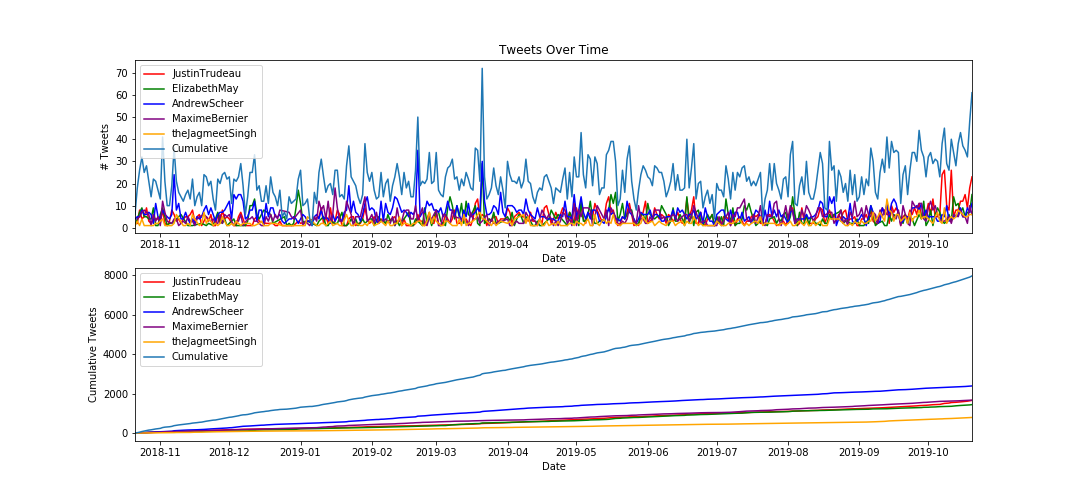
\includegraphics[scale=0.40]{figures/tweets_over_time}
  \caption[Daily and Cumulative Tweets over Time]{Daily and Cumulative Tweets over Time}
  \label{fig:tweets_over_time}
  \end{figure}


%Graph definition

\subsection{Topic Modeling}

\subsection{Topic Centrality}

\subsubsection{Eigenvector Centrality}

\subsubsection{Total Network Topic Centrality}

\subsubsection{Party Leader Topic Centrality}

\section{Results}

\subsection{Topic Saliency}

\subsection{Total Network Topic Centrality}

\subsection{Party Leader Topic Centrality}

\section{Discussion}

% RELATE BACK TO PUTNAM -> Talk about how bridging topics != hunky dory kind of
% discourse. Things can bridge party divides in toxic ways.

\bibliographystyle{plain}
\bibliography{bibliography}

\label{lastpage}

\end{document}

% end of NWSegui.tex